\chapter{XXE}

Un attacco XXE, detto anche XML External Entity, si riferisce a un tipo specifico di attacco Server-Side Request Forgery (SSRF) in base al quale un utente malintenzionato è in grado di accedere a file e servizi locali o remoti, abusando dell'errata configurazione del parser XML all'interno del codice di un'applicazione.\\ 

Quasi tutte le vulnerabilità degli attacchi XXE vengono riscontrate a causa di un endpoint API che accetta un payload XML (o simile a XML). Si potrebbe pensare che gli endpoint HTTP che accettano XML siano poco comuni (JSON), ma i formati simili a XML includono SVG, HTML/DOM, PDF (XFDF) e RTF. Questi formati simili a XML condividono molte somiglianze con le specifiche XML e, di conseguenza,
molti parser XML li accettano come input.\\

Il funzionamento di un attacco XXE risiede nel fatto che la specifica XML permette l'importazione di file esterni. Questa direttiva speciale, chiamata ``\textbf{external entity}'', viene interpretata dalla macchina su cui viene valutato il file XML. Ciò significa che un payload XML appositamente
realizzato e inviato al parser XML di un server potrebbe
comprometterne i file locali (come ad esempio /etc/shadow che memorizza credenziali importanti).

\newpage

\section{Direct XXE}
In ``direct XXE'', un oggetto XML viene inviato al server con un flag di entità esterna. Viene quindi analizzato e restituito un risultato che include tale entità.

\begin{figure}[H]
	\centering
	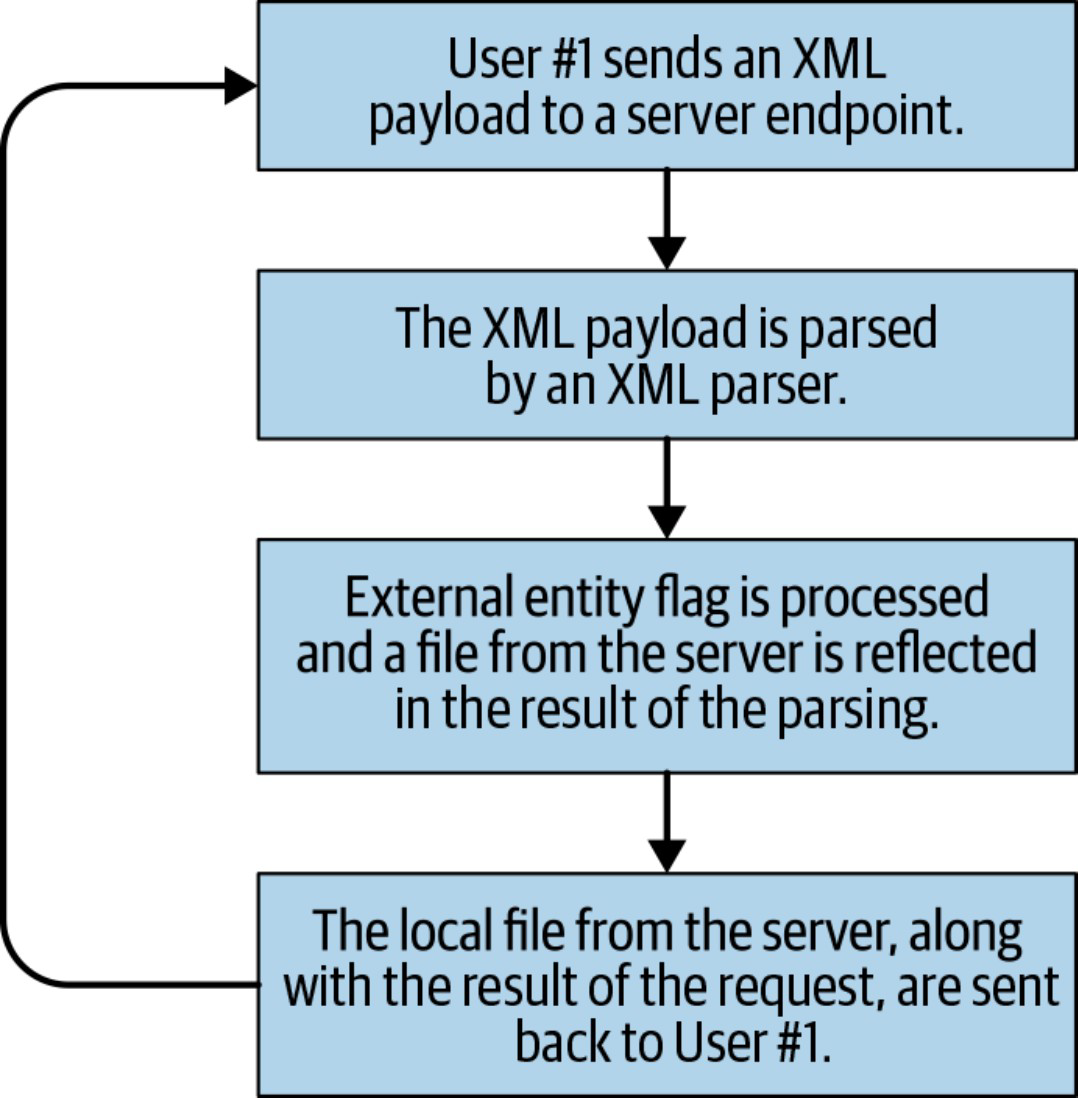
\includegraphics[width=7cm, keepaspectratio]{capitoli/web_security/imgs/direct_xxe_flow.png}
	\caption{Flow attacco ``direct XXE''.}
	\label{fig:direct_xxe_flow}
\end{figure}

\subsection{Esempio}
Immaginiamo che mega-bank.com abbia un'utilità di screenshot che ci permette di inviare schermate di ciò che accade nel portale della nostra banca direttamente all'assistenza clienti.

\begin{figure}[H]
	\centering
	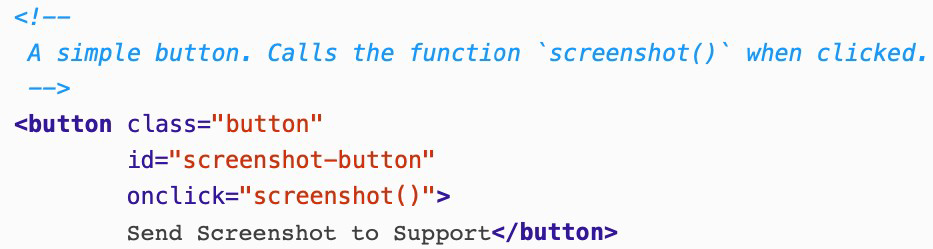
\includegraphics[width=12cm, keepaspectratio]{capitoli/web_security/imgs/xxe_banca_1.png}
	\label{fig:xxe_banca_1}
\end{figure}

\begin{figure}[H]
	\centering
	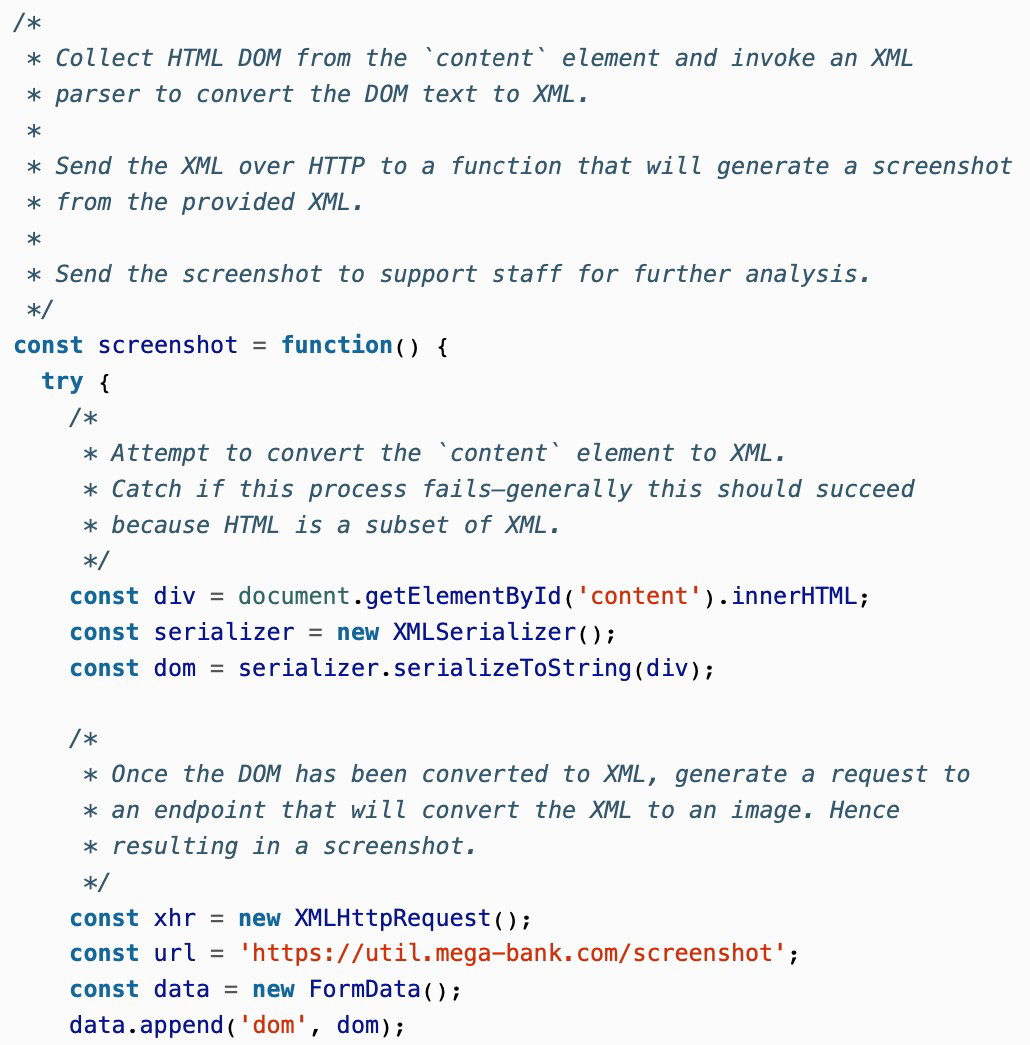
\includegraphics[width=10.5cm, keepaspectratio]{capitoli/web_security/imgs/xxe_banca_2.png}
	\caption{Frontend 1.}
	\label{fig:xxe_banca_2}
\end{figure}

\begin{figure}[H]
	\centering
	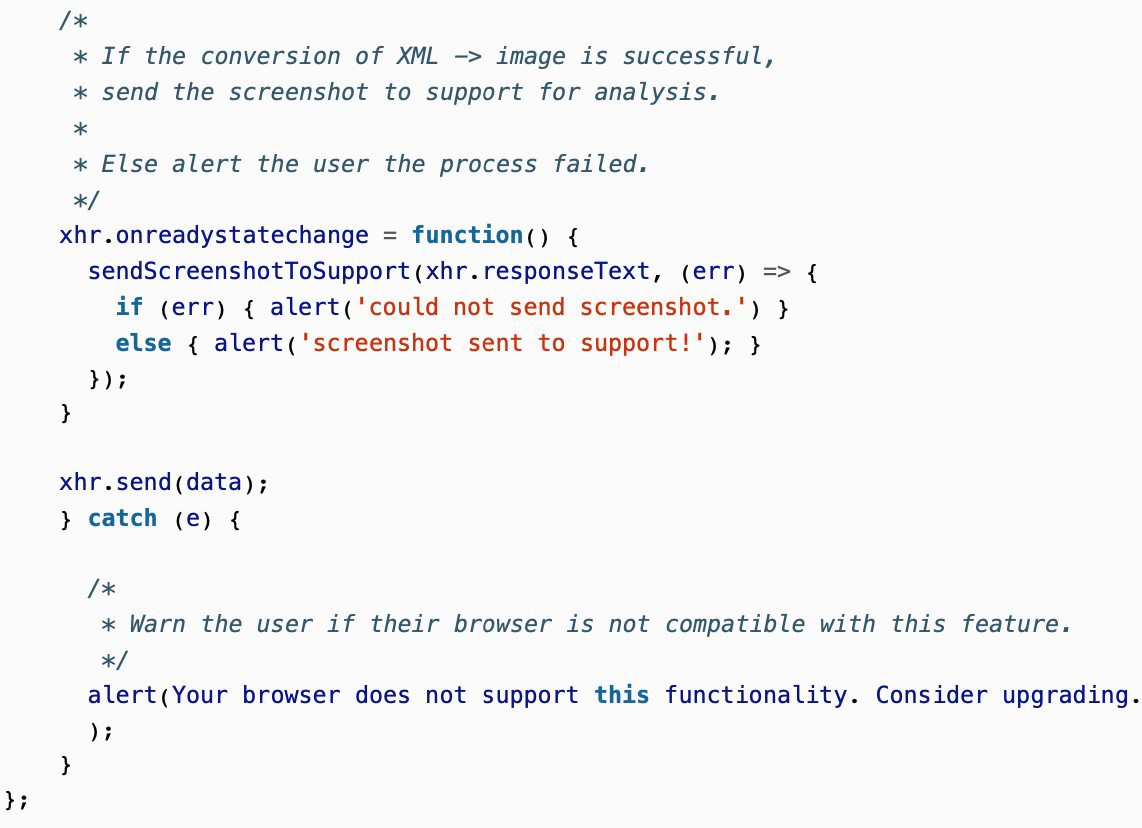
\includegraphics[width=10.5cm, keepaspectratio]{capitoli/web_security/imgs/xxe_banca_3.png}
	\caption{Frontend 2.}
	\label{fig:xxe_banca_3}
\end{figure}

\begin{figure}[H]
	\centering
	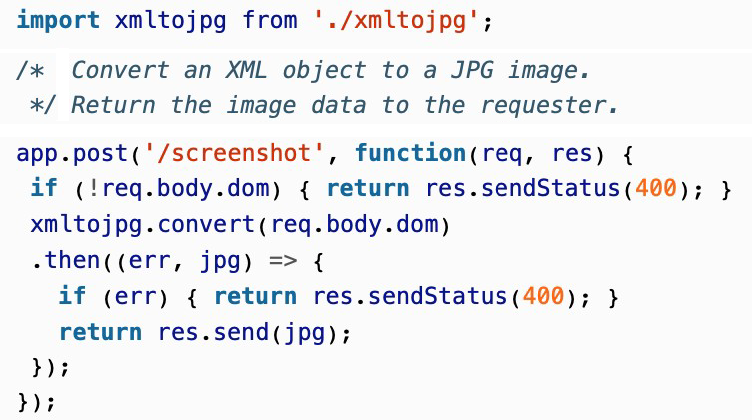
\includegraphics[width=8cm, keepaspectratio]{capitoli/web_security/imgs/xxe_banca_4.png}
	\caption{Backend.}
	\label{fig:xxe_banca_4}
\end{figure}

Come possiamo vedere, questo codice presenta più di un problema ma il più importante sicuramente è che potremmo chiamare noi stessi la funzione sendScreenshotToSupport() con le nostre immagini. Potremmo quindi falsificare la richiesta di rete e inviare al server il nostro payload personalizzato in cui cerchiamo di ottenere il file ``/etc/passwd'':
\begin{figure}[H]
	\centering
	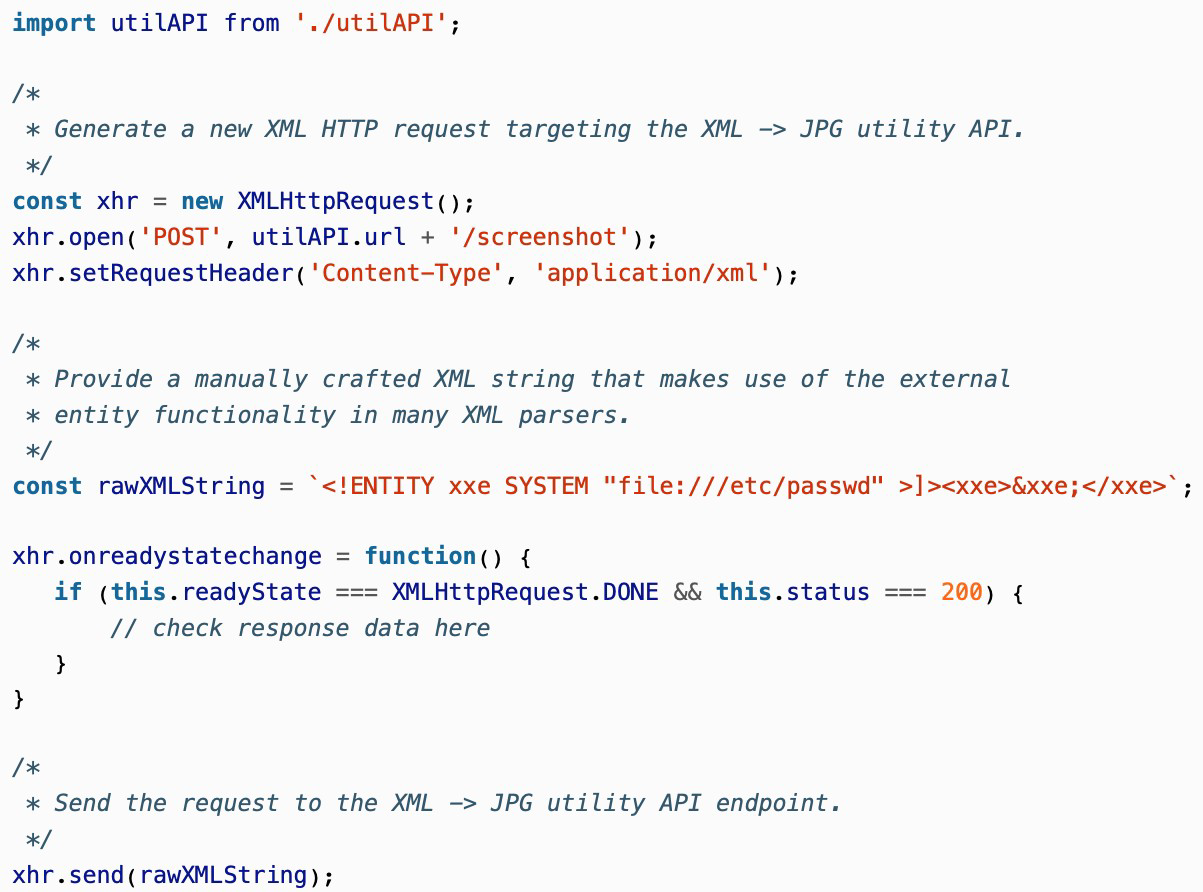
\includegraphics[width=12cm, keepaspectratio]{capitoli/web_security/imgs/xxe_banca_5.png}
	\caption{Payload XML.}
	\label{fig:xxe_banca_5}
\end{figure}

Se il parser XML non ha disabilitato esplicitamente le entità esterne, dovremmo vedere il contenuto del file richiesto all'interno della schermata restituita.

\newpage

\section{Indirect XXE}
A volte un attacco XXE può essere utilizzato contro un
endpoint che non opera direttamente su un oggetto XML
inviato dall'utente. Infatti, il fatto che un'API non prenda un oggetto XML come parte del suo payload non significa che non faccia uso di un parser XML.\\

In ``indirect XXE'', come risultato di una qualche forma
di richiesta, il server genera un oggetto XML. Tale oggetto include i parametri forniti dall'utente che possono portare all'inclusione di una ``external entity''.

\begin{figure}[H]
	\centering
	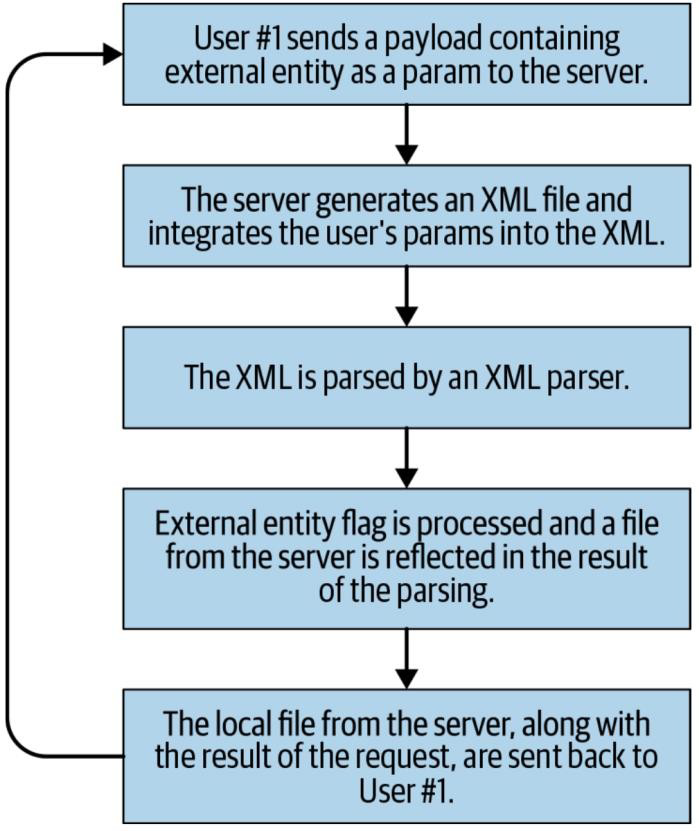
\includegraphics[width=8cm, keepaspectratio]{capitoli/web_security/imgs/indirect_xxe_flow.png}
	\caption{Flow attacco ``indirect XXE''.}
	\label{fig:indirect_xxe_flow}
\end{figure}

\newpage

\subsection{Esempio}

Si consideri il seguente caso d'uso. Uno sviluppatore sta scrivendo un'applicazione che richiede un solo parametro all'utente tramite un endpoint API REST. L'applicazione è progettata per sincronizzare questo parametro con un pacchetto software CRM di livello aziendale già in uso nell'azienda.

L'azienda CRM potrebbe aspettarsi payload XML per la sua API (Microsoft Dynamics CRM), il che significa che, sebbene l'endpoint esposto pubblicamente non accetti XML, per far sì che il server comunichi correttamente con il pacchetto software CRM, il payload dell'utente deve essere convertito in un oggetto XML tramite il server REST e quindi inviato al software CRM.\\

N.B. Per un hacker è facile capire se un'azienda usa XML o meno e la maggior parte delle volte lo usa. Questo perchè quando le aziende di software aziendale crescono, spesso aggiornano il loro software in modo frammentario piuttosto che costruirlo tutto da zero. Ciò significa che spesso le moderne API JSON/REST si interfacciano in un punto o nell'altro con un'API XML/SOAP.